\chapter{O Aplicativo}

O aplicativo ColetaCacau foi desenvolvido inicialmente pelo discente Henrique Serra Andrade e posteriormente pelo aluno Christian Menezes Oliveira. Este projeto atualizou as tecnologias do aplicativo existente e incorporou o RFID. Neste Capítulo está a descrição geral do aplicativo ColetaCacau e as atualizações realizadas.

\section{Arquitetura do Aplicativo}
O ColetaCacau foi desenvolvido utilizando a arquitetura \textit{Model-View-ViewModel (MVVM)}, amplamente recomendada para aplicativos móveis, por permitir uma separação clara entre a interface do usuário, a lógica de negócios e a manipulação dos dados \cite{Epiloksa2022EffectOM}. A escolha dessa arquitetura foi fundamental para manter o código organizado e facilitar futuras manutenções e expansões do sistema. A nova versão aprimorou a funcionalidade de coleta \textit{offline} já existente, incorporando tecnologias como o \textit{Redux Persist} para maior segurança no armazenamento temporário dos dados e o \textit{RealmDB} para sincronização otimizada e automática quando a conectividade é restaurada

A aplicação foi construída com \textit{Redux} para gerenciar o estado global e \textit{Redux Toolkit} para simplificar as operações comuns do \textit{Redux}, tornando o fluxo de dados previsível e o código mais conciso. Para armazenamento local e sincronização de dados \textit{offline}, utilizou-se o \textit{RealmDB}, uma base de dados orientada a objetos eficiente, ideal para uso em ambientes com baixa conectividade.

O sistema ColetaCacau utiliza um modelo de dados relacional para organizar as informações coletadas no campo. O diagrama de entidade-relacionamento (ER) representado na Figura \ref{fig:ClassDiagram01} mostra as principais entidades do sistema, sendo estas implementadas no aplicativo atráves do banco de dados \textit{offline} \textit{RealmDB}, incluindo propriedades, áreas homogêneas, unidades operacionais, pontos amostrais, árvores e coletas. Cada entidade está relacionada a outra de forma hierárquica, garantindo que os dados sejam armazenados de maneira estruturada e permitindo consultas eficientes sobre o progresso da safra e o estado das árvores.

\begin{figure}[htb]
    \centering
    \frame{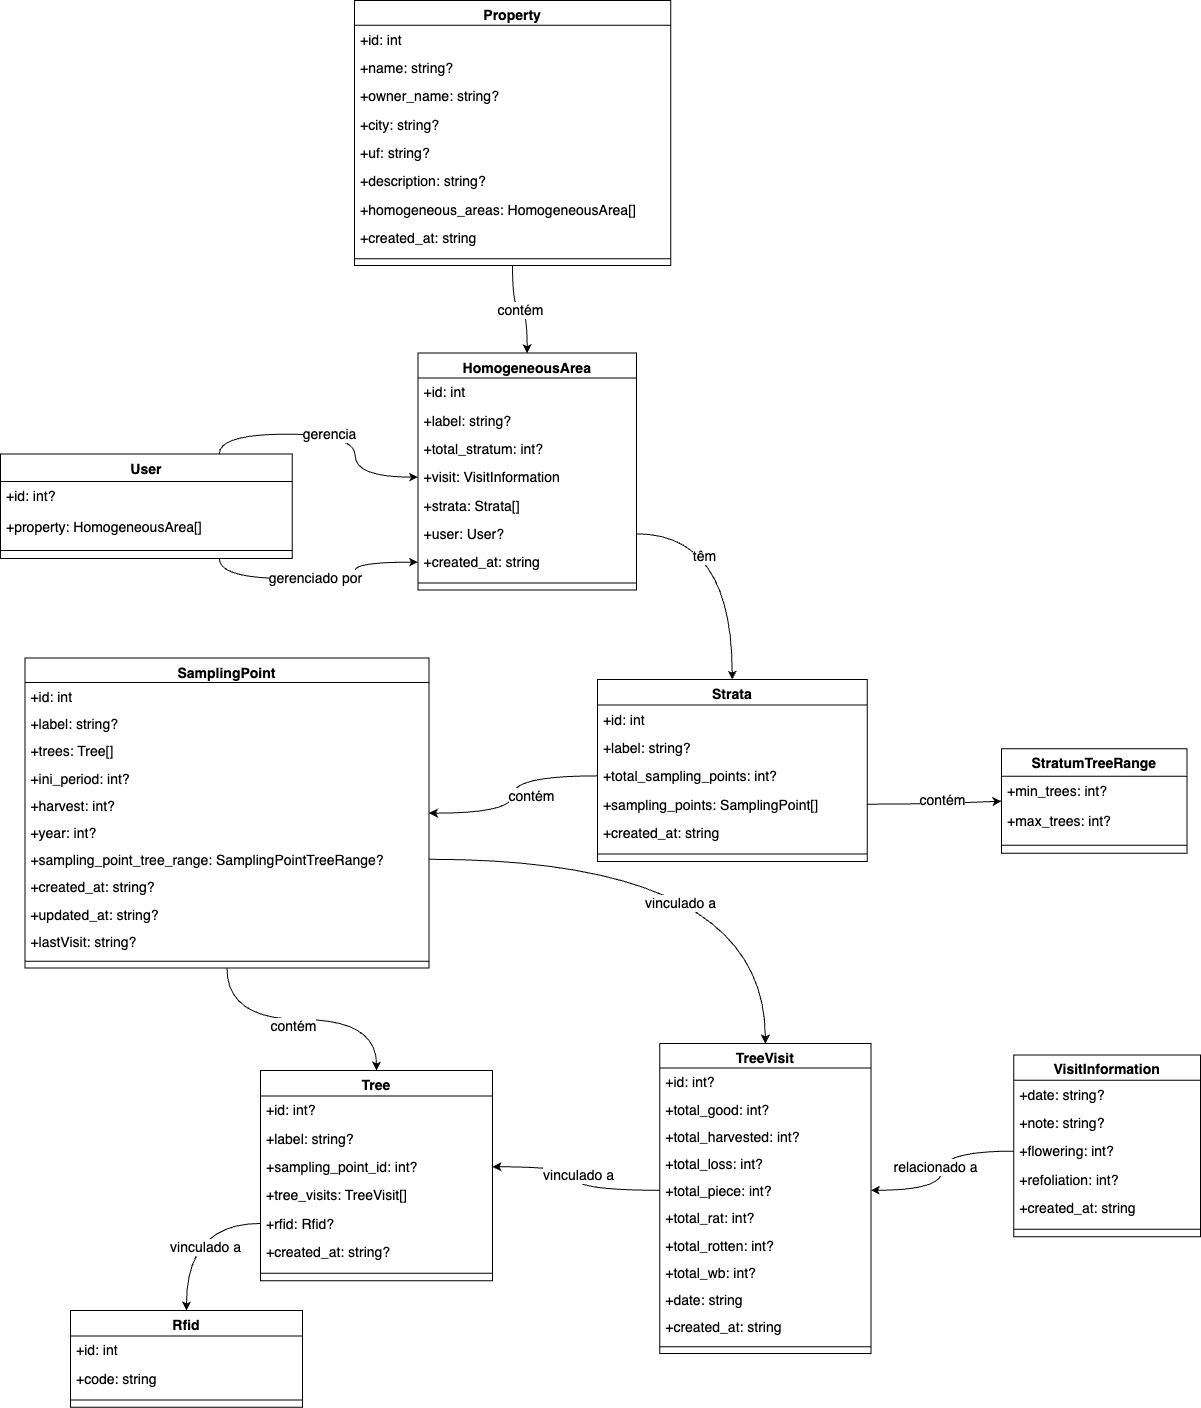
\includegraphics[width=\textwidth]{images/diagrams/class-diagram-p1.png}}
    \caption{Diagrama de classes das principais entidades do banco de dados \textit{offline}.}
    \label{fig:ClassDiagram01}
\end{figure}

\newpage 

A classe \textit{TreeVisit} armazena informações detalhadas sobre cada fruto, seguindo a metodologia estabelecida pela CEPLAC. No contexto das classes do \textit{RealmDB} implementadas no aplicativo, essa classe é modelada como é apresentado na Figura \ref{fig:ClassDiagram02}:

\begin{figure}[htb]
 \centering
 \frame{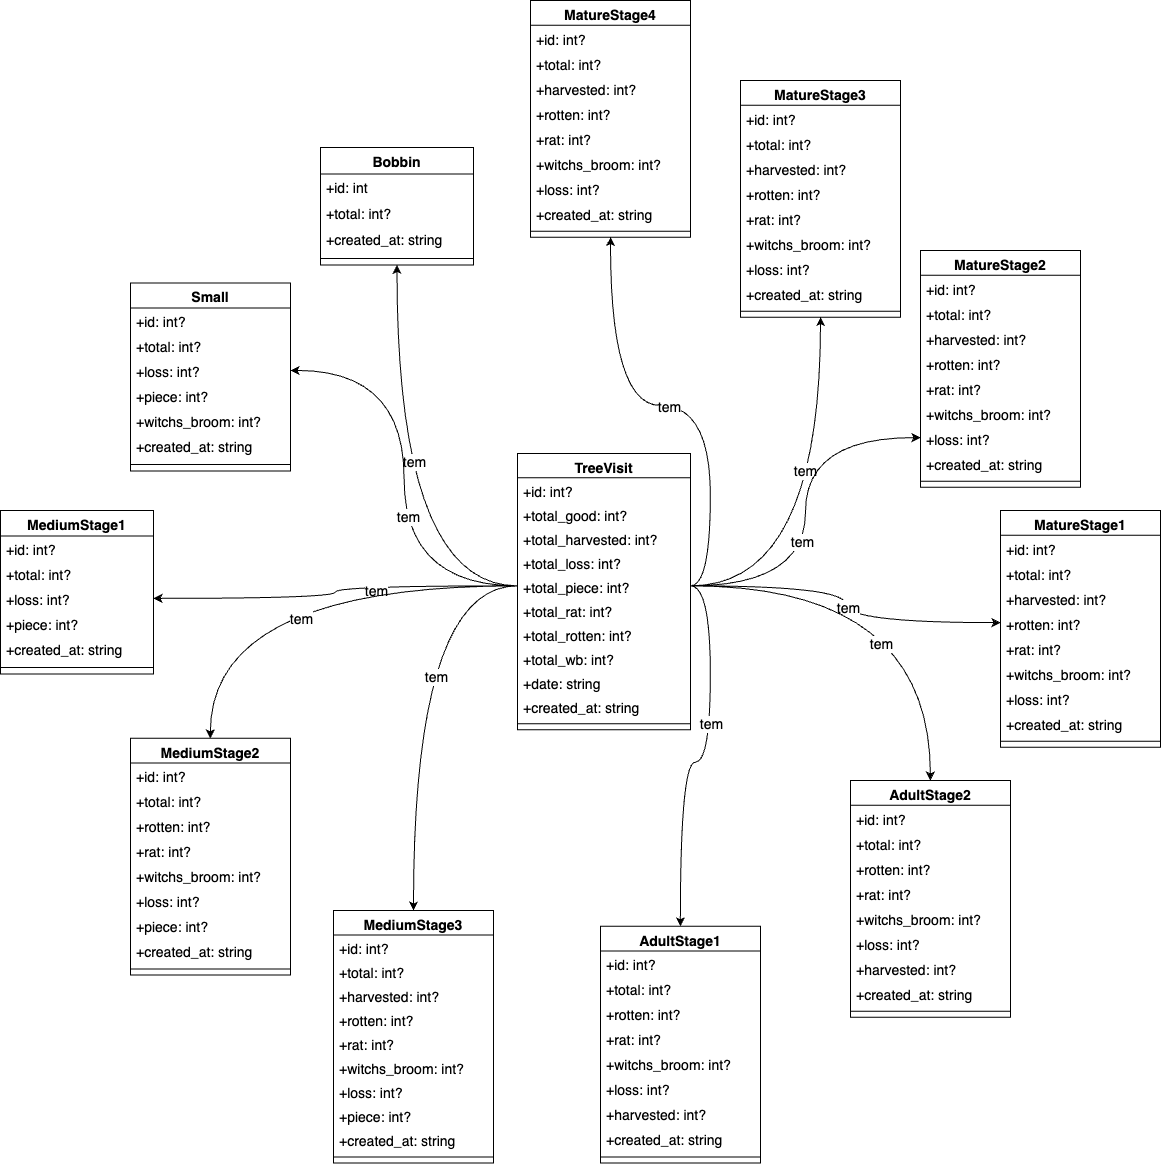
\includegraphics[width=\textwidth]{images/diagrams/class-diagram-p2.png}}
 \caption{Diagrama de classes do banco de dados \textit{offline} para os dados dos frutos.}
 \label{fig:ClassDiagram02}
\end{figure}

\newpage

\section{Integração com RFID}
A tecnologia RFID foi implementada para otimizar a identificação e monitoramento das árvores amostradas no ColetaCacau. Cada árvore recebe uma tag RFID, que contém um identificador único. Durante a coleta, o coletor utiliza o aplicativo para ler essas tags e associar os dados coletados à árvore correta.

\subsection{Processo de Implementação do RFID}
\begin{enumerate}
    \item \textbf{Leitura das Tags:} Um leitor RFID integrado ao dispositivo móvel lê a tag associada a uma árvore. O aplicativo, por meio de bibliotecas \textit{JavaScript} compatíveis com \textit{React Native}, interpreta essa leitura e exibe as informações da árvore diretamente na interface do usuário. Esse processo elimina a necessidade de o coletor identificar manualmente as árvores, reduzindo os erros e aumentando a precisão da coleta de dados. Um módulo nativo implementado em \textit{Kotlin} foi criado para atuar como um \textit{listener} verificando se existe algum dispositivo conectado ao celular e se este dispositivo é um leitor compátivel com a aplicação.

    \item \textbf{Associação com Dados Amostrais:} Assim que uma árvore é identificada via RFID, o aplicativo exibe as informações pré-existentes da árvore e permite que o coletor insira novos dados, como número de frutos ou condições da planta. Esses dados são armazenados localmente até que uma conexão à internet esteja disponível para sincronização com o servidor. O aplicativo identifica quando há uma conexão com internet e habilita o botão de envio de dados, que permite ao coletor enviar os dados que foram coletados.

    \item \textbf{Monitoramento de Erros com RFID:} A integração com o Sentry também monitora a estabilidade do sistema de leitura de tags RFID e de todo o aplicativo, garantindo que falhas sejam reportadas e corrigidas rapidamente, melhorando a confiabilidade do aplicativo.
\end{enumerate}

\section{Funcionalidades Desenvolvidas}

\subsection{Aprimoramento do Armazenamento \textit{Offline}}
A funcionalidade de coleta \textit{offline} do ColetaCacau, essencial para operação em áreas com baixa ou nenhuma conectividade e que já estava desenvolvida no aplicativo, foi aprimorada para oferecer maior segurança, integridade e eficiência no gerenciamento dos dados coletados. Nesta nova versão, o aplicativo se destaca por sua capacidade de armazenar informações localmente de maneira robusta, seguindo os padrões estabelecidos pela nova documentação do \textit{RealmDB}.

O \textit{RealmDB} foi aprimorado para oferecer desempenho superior no armazenamento local de dados, permitindo a coleta de grandes volumes de informações diretamente no dispositivo do coletor. Essa abordagem assegura que as informações sejam protegidas e prontamente disponíveis, mesmo em locais remotos.

\subsection{Gestão de Dados com \textit{Redux Toolkit}}
O \textit{Redux Toolkit} foi implementado para facilitar o gerenciamento de estado em todo o aplicativo, promovendo um fluxo de dados previsível e eficiente. Ele simplifica a definição de \textit{reducers}, \textit{actions} e a criação da \textit{store}, tornando a arquitetura do aplicativo mais robusta e escalável.

O \textit{Redux Persist} foi integrado ao sistema para garantir que o estado da aplicação seja preservado entre sessões, mesmo que o aplicativo seja fechado e reaberto. Isso assegura que os dados coletados no campo não sejam perdidos.

Atualmente, o ColetaCacau possui uma larga quantidade de dados, que é requisitada ao realizar o login no aplicativo. A utilização desta biblioteca alinhado ao uso do banco de dados \textit{offline} permite maior eficiência na manipulação destes dados.

\subsection{Monitoramento de Erros}
A integração com o \textit{Sentry} foi uma adição crucial ao sistema para garantir a estabilidade do aplicativo. O \textit{Sentry} monitora erros e exceções em tempo real, oferecendo relatórios detalhados sobre falhas que podem ocorrer no aplicativo, seja por incompatibilidade de dispositivos ou problemas de lógica de programação.

\begin{itemize}
    \item \textbf{Relatórios Automáticos:} Sempre que ocorre um erro no aplicativo, é gerado automaticamente um relatório que inclui detalhes técnicos sobre a falha, como a linha de código afetada, o tipo de erro e o dispositivo em que ocorreu.

    \item \textbf{Correção Proativa de Bugs:} Com base nos relatórios gerados por esta ferramenta, a equipe de desenvolvimento pode identificar rapidamente as falhas e liberar atualizações corretivas. Isso é especialmente importante para evitar a interrupção da coleta de dados em campo, onde o tempo é um recurso crítico.
\end{itemize}

\subsection{Atualização de Bibliotecas e \textit{Frameworks}}
Uma etapa essencial no aprimoramento do ColetaCacau foi a atualização do \textit{React Native} para a versão 0.76, descrita na documentação oficial do framework\footnote{\url{https://reactnative.dev/blog/2024/10/23/release-0.76-new-architecture}}. Essa atualização visou não apenas garantir compatibilidade com os sistemas operacionais móveis mais recentes, mas também trazer melhorias significativas na performance, segurança e eficiência do aplicativo.

Com a migração para a nova versão, houve uma redução substancial no tamanho final do aplicativo. Essa melhoria foi alcançada por meio de otimizações no código-base e pela remoção de dependências obsoletas, tornando o ColetaCacau mais leve e fácil de instalar, especialmente importante para usuários em áreas rurais com conectividade limitada. Além disso, o gerenciamento de memória foi aprimorado, o que resultou em uma navegação mais fluida e em uma melhor experiência para o usuário, mesmo em dispositivos com hardware modesto.

Outro benefício relevante foi o suporte ampliado para funcionalidades dos sistemas operacionais mais modernos, como melhorias na gestão de permissões e maior integração com bibliotecas essenciais, como o \textit{RealmDB} e o \textit{Redux}, garantindo a estabilidade e a robustez do aplicativo. Durante o processo de atualização, ajustes foram realizados no código para adaptar funcionalidades às mudanças da \textit{API} do \textit{React Native}, incluindo a substituição de métodos descontinuados e a reestruturação de componentes de interface. Esses ajustes asseguraram que o aplicativo estivesse alinhado às melhores práticas recomendadas.

Essas mudanças não apenas tornaram o aplicativo mais eficiente, mas também reforçaram sua estabilidade e capacidade de atender às necessidades dos coletores em campo, posicionando o ColetaCacau como uma solução tecnológica confiável e adaptada ao contexto da agricultura de precisão.

\section{Interface com o Usuário}
A interface do ColetaCacau foi projetada para ser simples e intuitiva, com uma navegação linear que facilita o uso em campo. O fluxo de navegação do aplicativo segue uma hierarquia clara, levando o usuário passo a passo desde o cadastro das propriedades até a coleta dos dados das árvores específicas.

\subsection{Fluxo de Navegação Linear do Aplicativo}
\begin{itemize}
    \item \textbf{Propriedades:} O processo começa com a listagem de propriedades cadastradas. Cada propriedade contém diversas áreas homogêneas. Cada propriedade é vinculada à um ou mais coletores.

    \item \textbf{Áreas Homogêneas:} Após selecionar uma propriedade, o usuário navega para as áreas homogêneas. Cada área homogênea é uma subdivisão que representa grandes regiões com características similares de solo, clima ou uso da terra.

    \item \textbf{Unidades Operacionais:} Dentro de cada área homogênea, há subdivisões chamadas de unidades operacionais, que representam setores menores, como blocos de uma fazenda. Ao selecionar uma unidade operacional, o usuário tem duas opções de navegação:
    \begin{itemize}
        \item \textbf{Dados da Prática:} O usuário pode optar por registrar dados gerais sobre o estado da área, como refoliação, floração, presença de pragas (como ratos e insetos), inundações, entre outros. Esses dados refletem a condição atual da área e ajudam no acompanhamento geral da plantação.

        \item \textbf{Pontos Amostrais:} Alternativamente, o usuário pode escolher navegar até os pontos amostrais, onde a coleta detalhada dos dados da árvore será realizada.
    \end{itemize}

    \item \textbf{Pontos Amostrais:} Ao acessar a lista de pontos amostrais, o coletor tem acesso às localizações específicas dentro das unidades operacionais, onde será realizada a coleta de dados mais detalhada. Cada ponto amostral contém várias árvores que são monitoradas individualmente.

    \item \textbf{Árvores:} Dentro de cada ponto amostral, o coletor verá a lista de árvores associadas. A integração com RFID facilita a identificação automática das árvores, permitindo que o coletor seja direcionado exatamente para a árvore correta, sem a necessidade de identificação manual.

    \item \textbf{Coleta dos Dados da Árvore:} Após a identificação da árvore, o usuário acessa a tela de coleta de dados específicos para cada árvore. Nessa tela, são registrados dados sobre o fruto do cacau, separados por estágios de desenvolvimento conforme o tempo (em dias) desde o último estágio de maturação.
    
    Estágios de Desenvolvimento do Fruto:
    \begin{itemize}
        \item 0 a 21 dias: Bilro
        \item 21 a 42 dias: Pequeno
        \item 42 a 63 dias: Médio
        \item 63 a 84 dias: Médio Estágio 2
        \item 84 a 105 dias: Médio Estágio 3
        \item 105 a 126 dias: Adulto
        \item 126 a 147 dias: Adulto Estágio 2
        \item 147 a 168 dias: Maduro
        \item 168 a 189 dias: Maduro Estágio 2
        \item 189 a 210 dias: Maduro Estágio 3
        \item Acima de 210 dias: Maduro Estágio 4
    \end{itemize}
\end{itemize}

Cada estágio representa uma fase específica no crescimento do fruto do cacau. O aplicativo permite que o coletor registre as informações de cada estágio, garantindo um acompanhamento detalhado e preciso da evolução da safra. Dados como quantidade de frutos, perdas e qualidade são registrados e vinculados ao estágio correspondente.

A arquitetura do ColetaCacau foi desenvolvida utilizando uma abordagem modular, garantindo que cada parte do sistema funcione de forma independente, mas integrando-se de maneira eficiente. O diagrama de componentes apresentado na Figura \ref{fig:ComponentsDiagram} ilustra como as diferentes partes do sistema, como o módulo de leitura de RFID, o gerenciamento de dados \textit{offline} e a interface do usuário, estão organizadas e interagem para garantir a funcionalidade completa do aplicativo.

\newpage 

\begin{figure}[htb]
    \centering
    \frame{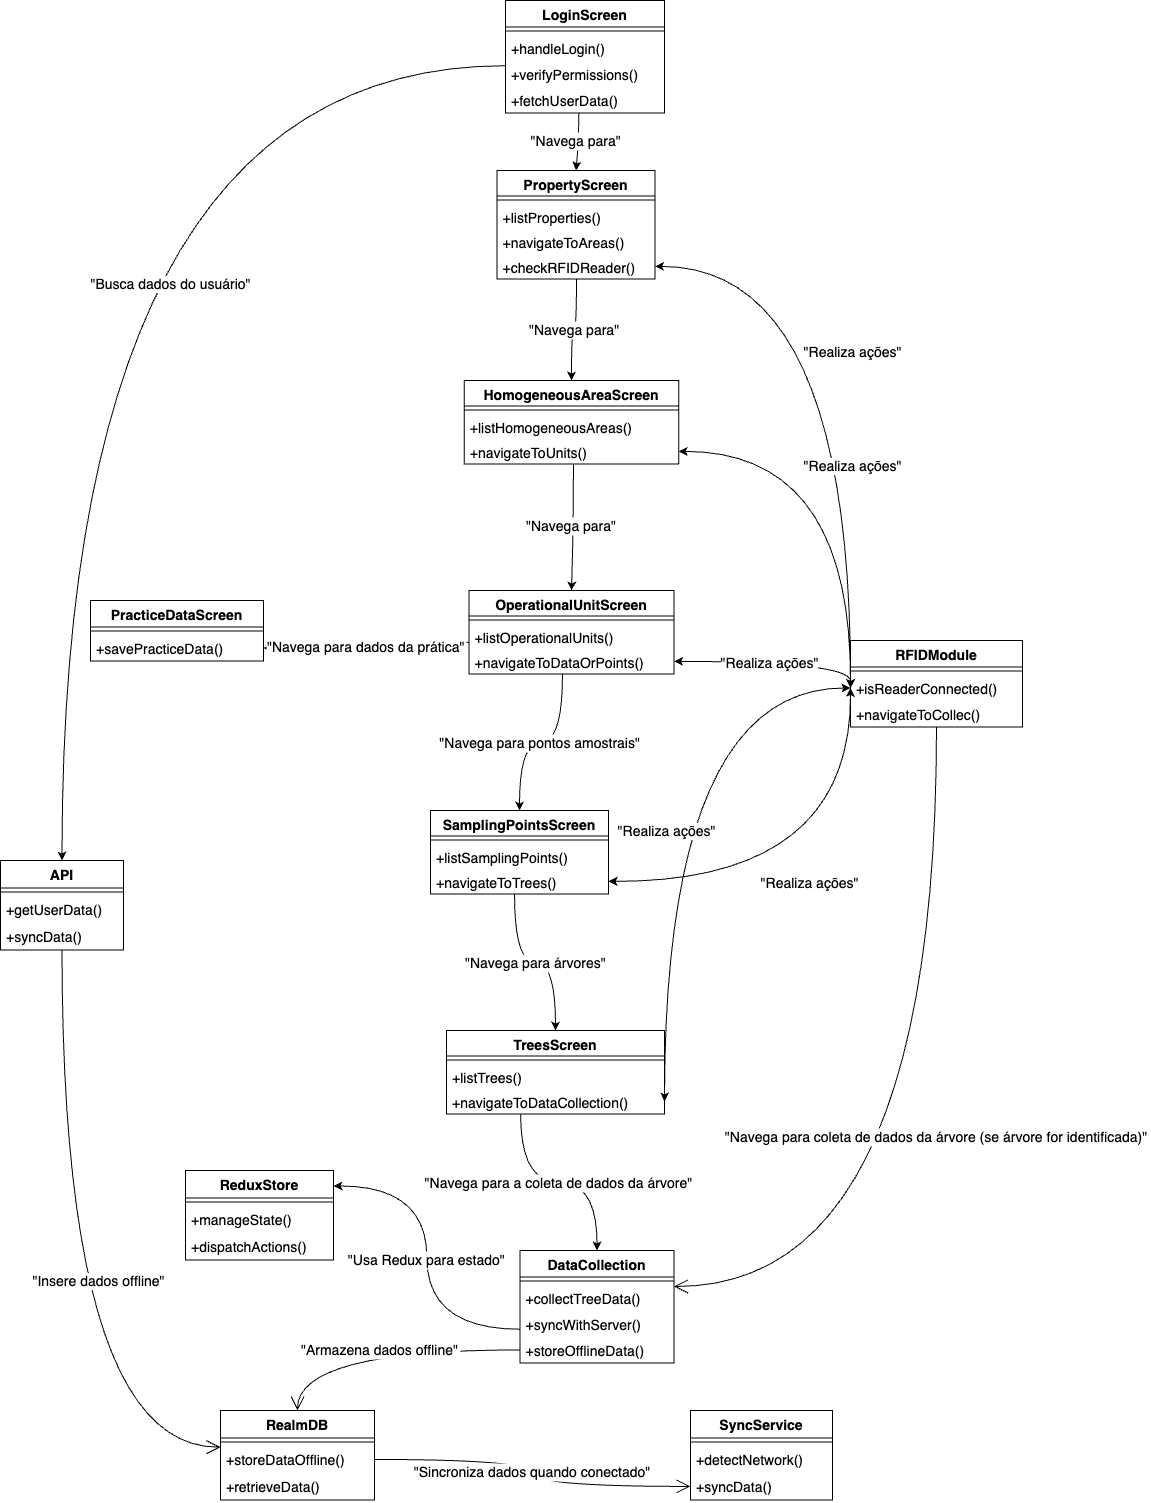
\includegraphics[width=\textwidth]{images/diagrams/components-diagram.png}}
    \caption{Diagrama de componentes.}
    \label{fig:ComponentsDiagram}
\end{figure}

\newpage

\subsection{\textit{Design} e Usabilidade}
O \textit{design} do ColetaCacau prioriza a simplicidade e a clareza. Cada passo do fluxo de navegação é apresentado de maneira clara e linear, o que facilita a operação por coletores que podem ter pouca familiaridade com tecnologia.

A interface também foi otimizada para garantir uma boa performance mesmo em dispositivos com \textit{hardware} limitado, uma realidade comum nas áreas rurais onde o aplicativo será utilizado.

\begin{itemize}
    \item \textbf{Telas organizadas:} As informações são exibidas em listas simples e fáceis de navegar, com botões de grande visibilidade que facilitam a interação.

    \item \textbf{Navegação intuitiva:} A hierarquia das telas segue a estrutura lógica da coleta de dados, o que facilita o uso em campo, mesmo em situações de pressão ou limitações de tempo.

    \item \textbf{Responsividade:} A interface foi projetada para ser responsiva e se adaptar a diferentes tamanhos de tela, garantindo uma experiência consistente tanto em smartphones quanto em tablets.
\end{itemize}

A Figura \ref{fig:CollectScreenTablet} mostra a visualização da tela de coleta de dados do cacau em um tablet, enquanto a Figura \ref{fig:CollectScreenPhone} demonstra a mesma tela adaptada para um smartphone, evidenciando a responsividade do \textit{design}.

\begin{figure}[H]
    \centering
    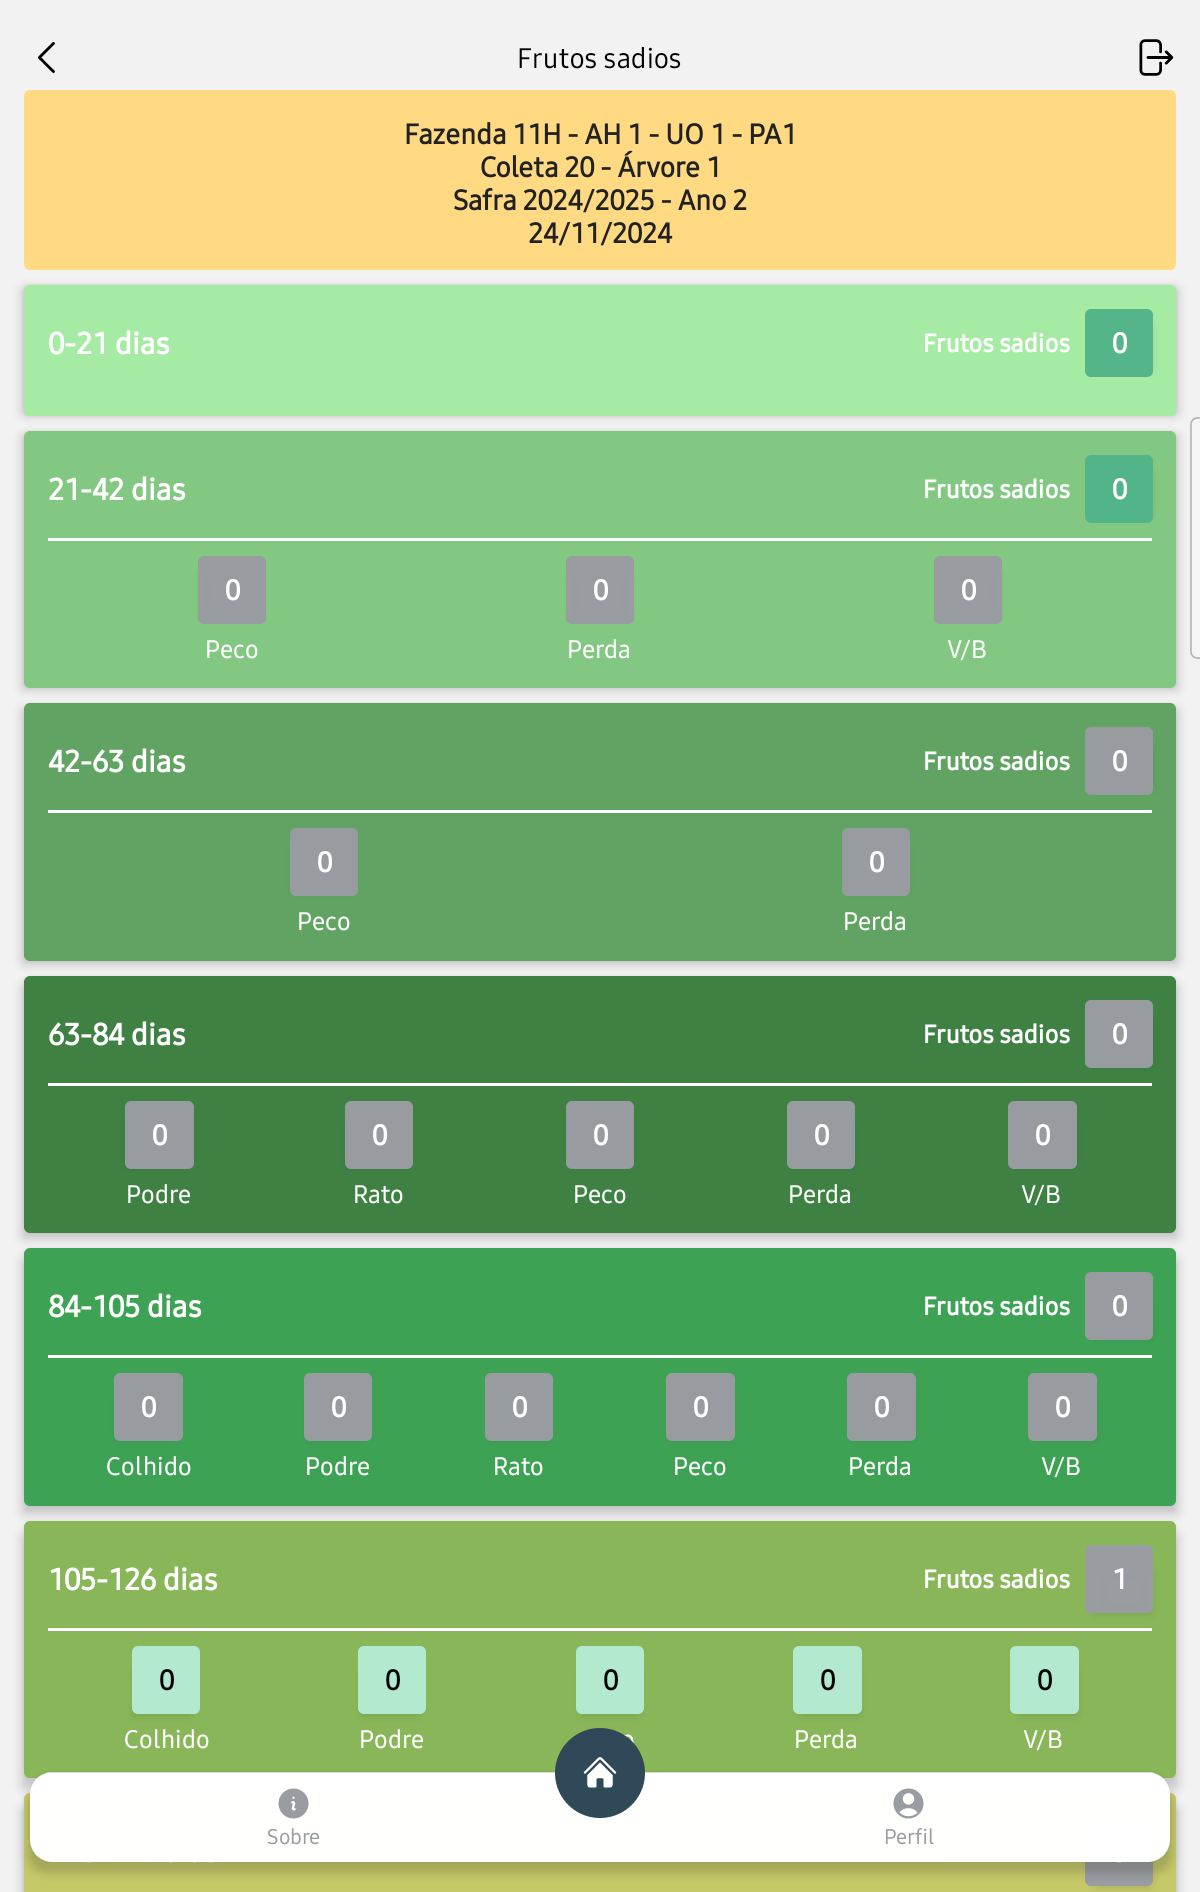
\includegraphics[width=0.4\textwidth]{images/app/collect-screen-tablet.png}
    \caption{Tela da coleta de dados em um \textit{tablet}.}
    \label{fig:CollectScreenTablet}
\end{figure}
\newpage
\begin{figure}[H]
    \centering
    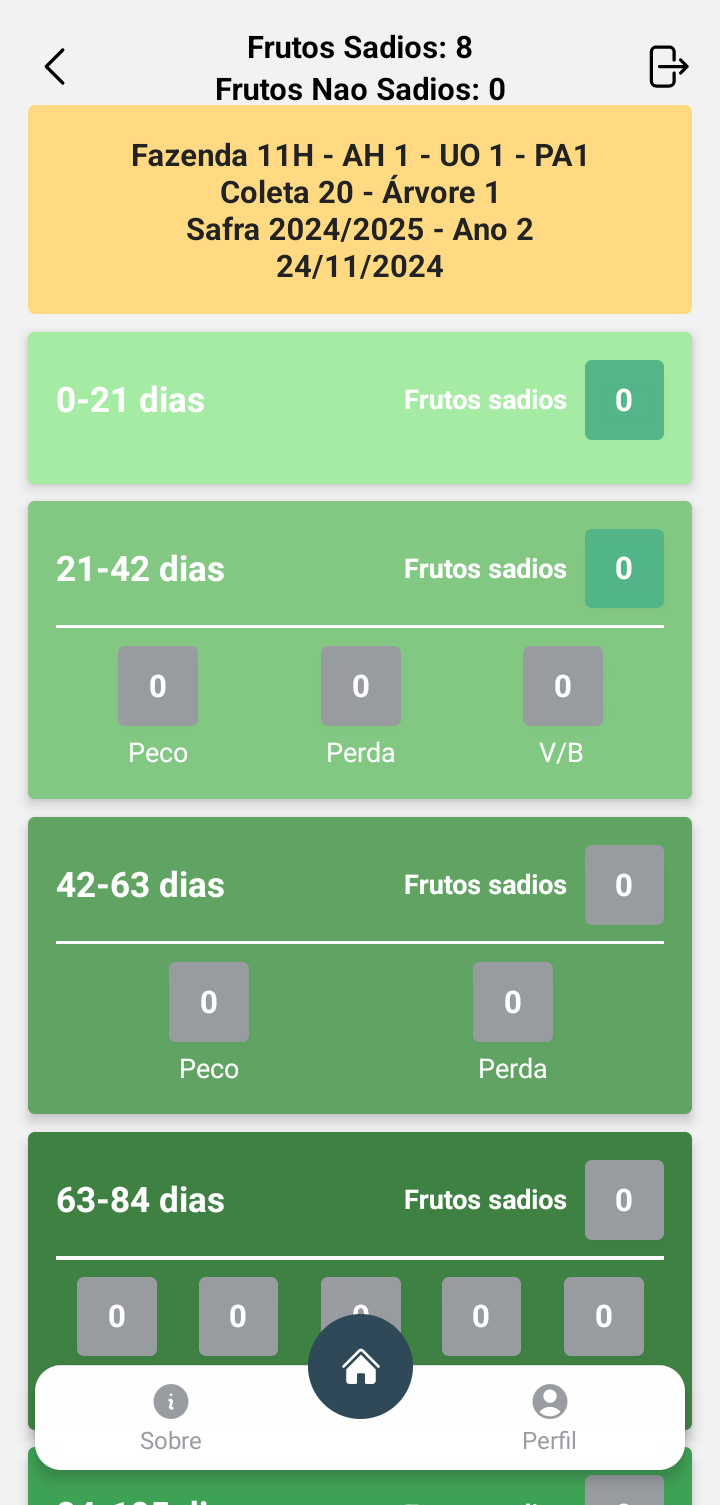
\includegraphics[width=0.4\textwidth]{images/app/collect-screen-phone.png}
    \caption{Tela da coleta de dados em um \textit{smartphone}.}
    \label{fig:CollectScreenPhone}
\end{figure}

Essa abordagem responsiva reforça o compromisso do ColetaCacau em oferecer uma experiência de usuário acessível e eficiente, independentemente do dispositivo utilizado no campo.

\subsection{Fluxo de Coleta e Operação}
A Figura \ref{fig:SequenceDiagram} representa o diagrama de sequência que descreve o processo de coleta de dados no ColetaCacau, desde o momento em que o coletor faz a leitura da tag RFID até o armazenamento dos dados localmente e a sincronização com o servidor. O diagrama detalha a interação entre os componentes principais do sistema — usuário, aplicativo, banco de dados \textit{offline} e servidor central —, mostrando o fluxo de operação e as etapas necessárias para garantir que os dados coletados sejam registrados corretamente e disponibilizados para análise.

\begin{figure}[htb]
 \centering
 \frame{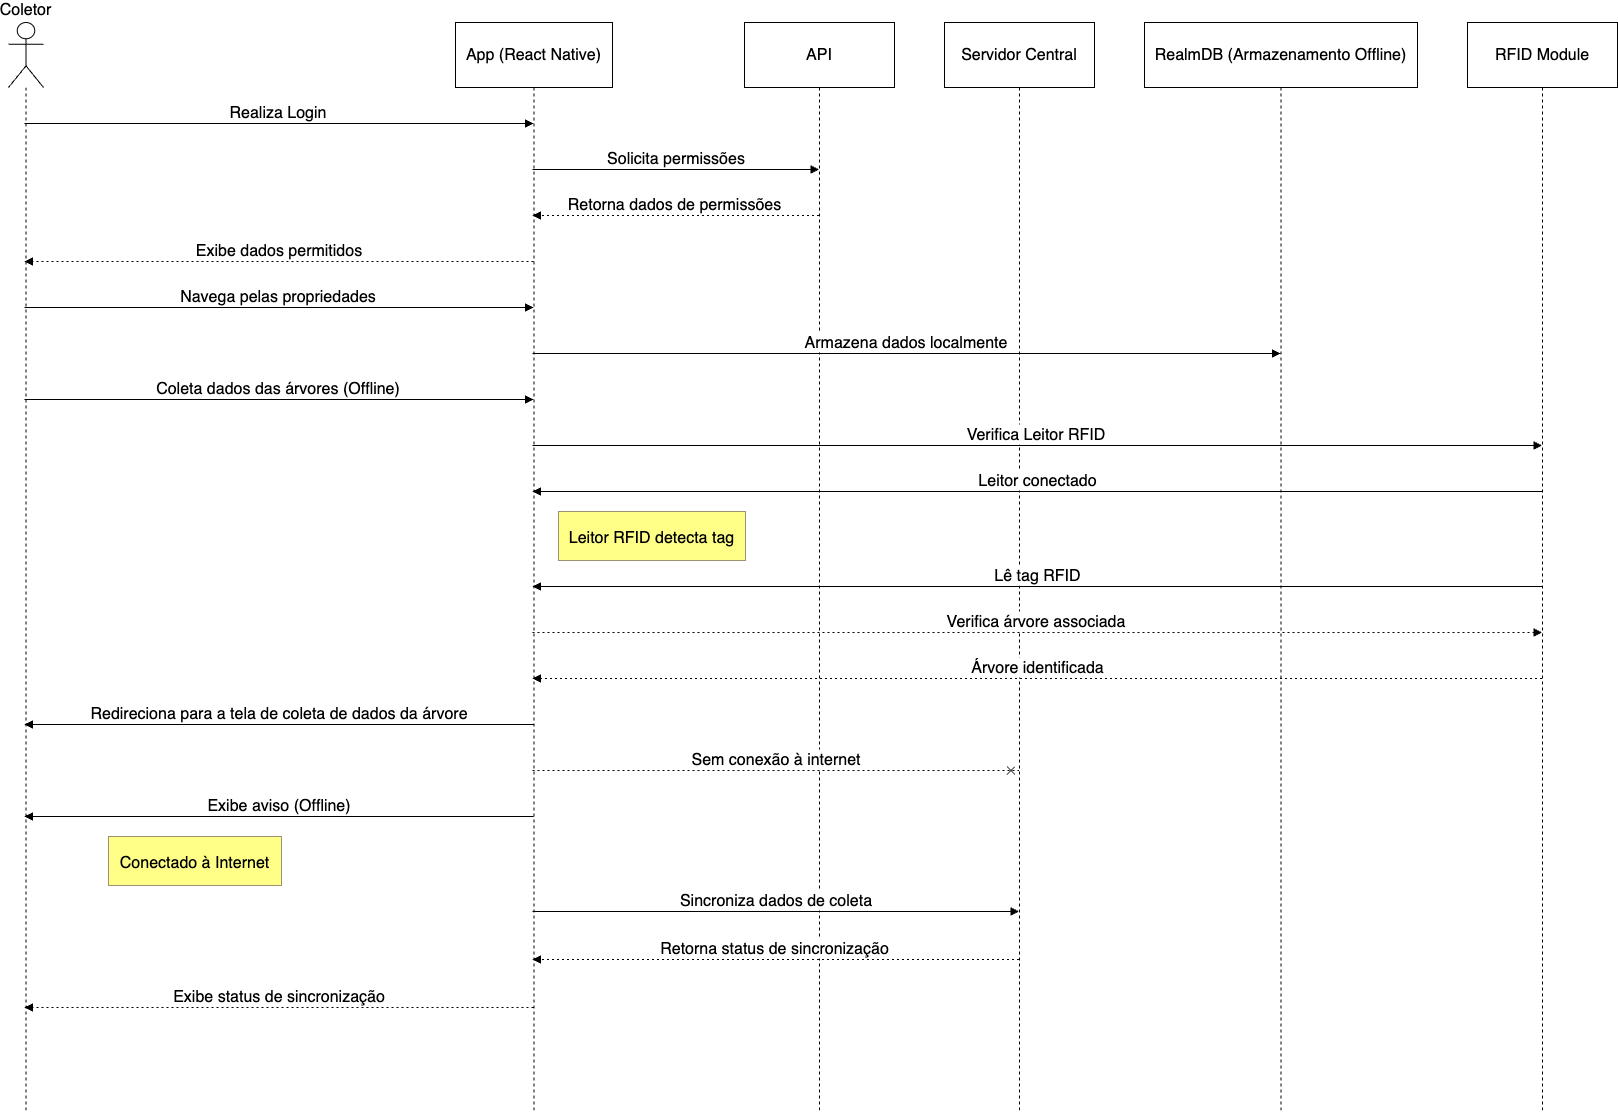
\includegraphics[width=\textwidth]{images/diagrams/sequence-diagram.png}}
 \caption{Diagrama de sequência.}
 \label{fig:SequenceDiagram}
\end{figure}

Para fornecer feedback visual ao coletor sobre a prontidão do aplicativo para realizar leituras de tags RFID, foi implementado um indicador no canto inferior direito de todas as telas de listagem. Esse indicador permite que o coletor saiba, em tempo real, se o leitor está ativo e pronto para captar informações de uma tag RFID, promovendo uma experiência mais fluida e intuitiva durante a coleta de dados.

A Figura \ref{fig:RfidReaderIndicator} ilustra os dois estados possíveis do indicador: no estado inativo, o leitor não está preparado para realizar a leitura; no estado ativo, o aplicativo está pronto para capturar as informações de uma tag, sinalizando de forma clara e acessível ao usuário. Essa funcionalidade reduz incertezas durante a operação e garante maior eficiência no processo de coleta.

\begin{figure}[H]
    \centering
    \begin{minipage}[b]{0.40\textwidth}
        \centering
        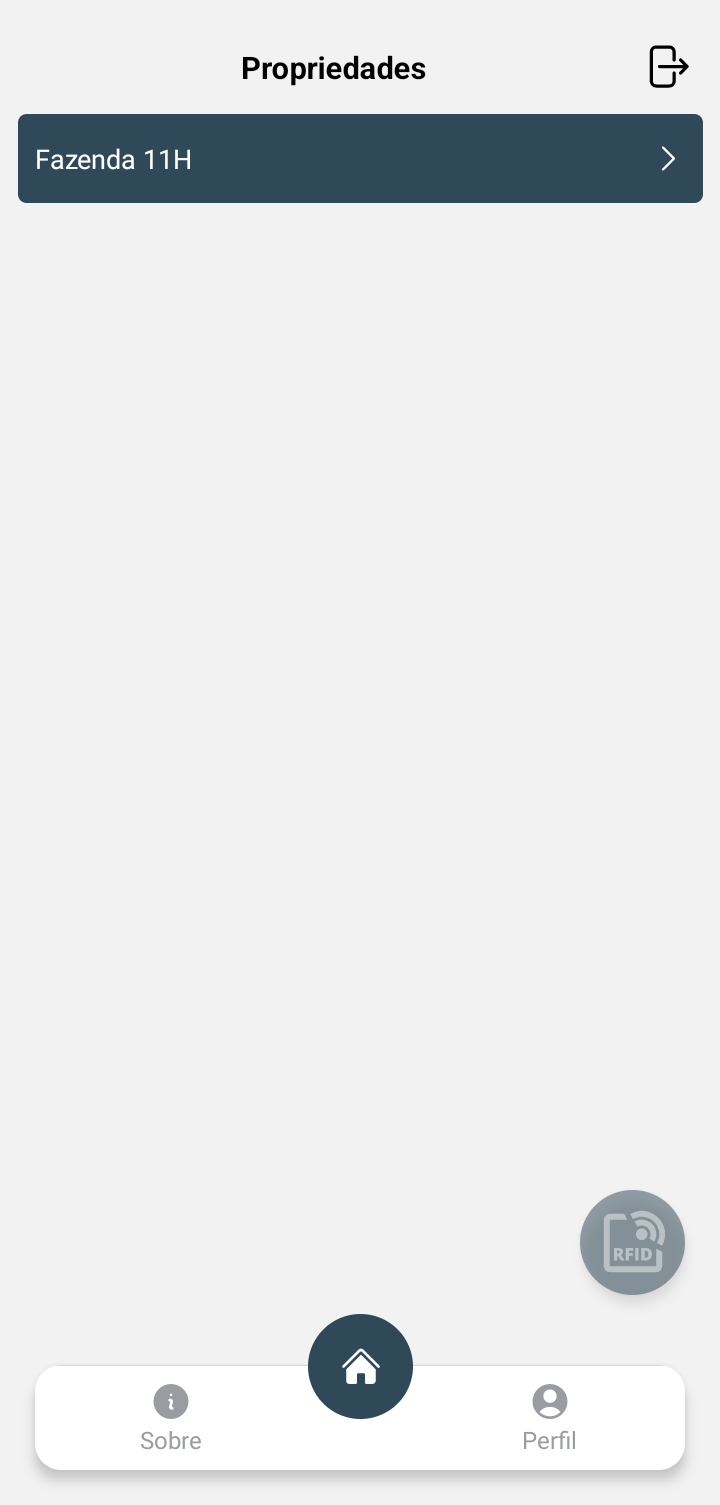
\includegraphics[width=\textwidth]{images/app/rfid-disabled.png}
        \caption*{(a) Indicador de leitura de tags em estado inativo.}
    \end{minipage}
    \hspace{5pt}
    \begin{minipage}[b]{0.40\textwidth}
        \centering
        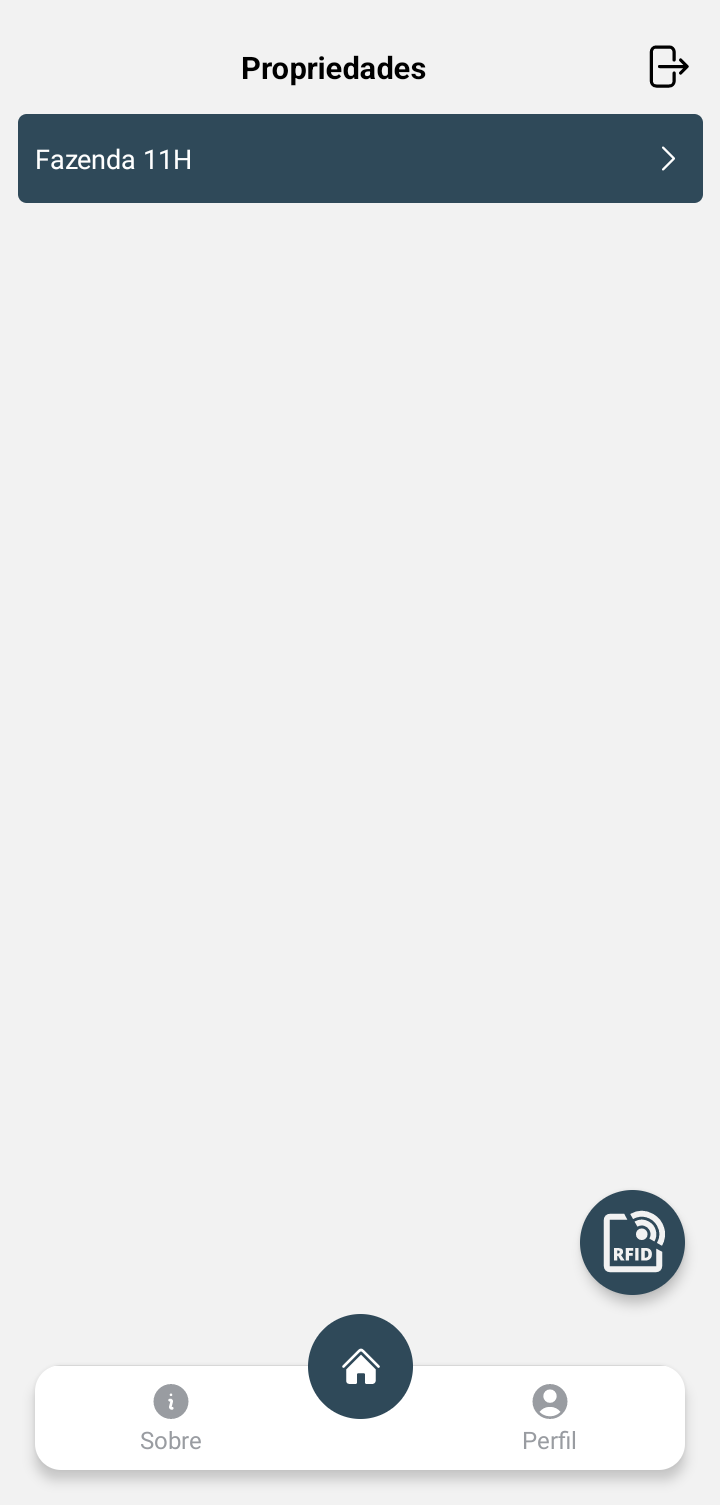
\includegraphics[width=\textwidth]{images/app/rfid-enabled.png}
        \caption*{(a) Indicador de leitura de tags em estado ativo.}
    \end{minipage}
    \hspace{5pt}
    
    \caption{Leitor RFID em dois estados: (a) Normal e (b) Ativo durante a leitura de uma tag.}
    \label{fig:RfidReaderIndicator}
\end{figure}

\newpage
